\begin{table}[H]
    \centering
    \begin{minipage}{0.45\textwidth}
        \centering
        \caption{\textit{Exp1: Measured resistance, voltage, and current for the water electrolyzer.}}
        \renewcommand{\arraystretch}{1.4} % Adjust row height
        \setlength{\tabcolsep}{8pt} % Adjust column spacing
        \begin{tabular}{|c|c|c|}
            \hline
            \textbf{R (\si{\ohm})} & \textbf{U (\si{\volt})} & \textbf{I (\si{\ampere})} \\
            \hline
            0 & 0 & 0 \\
            \hline
            0.1 & 0.105 & 0 \\
            \hline
            0.33 & 0.67 & 0 \\
            \hline
            1 & 1.43 & 0 \\
            \hline  
            3.3 & 3.19 & 0.24 \\
            \hline
            10 & 3.52 & 0.8 \\
            \hline
            33 & 3.64 & 1.04 \\
            \hline
            100 & 3.68 & 1.1 \\
            \hline
            330 & 3.69 & 1.14 \\
            \hline
        \end{tabular}
        \label{tab:exp1_results}
    \end{minipage}
    \hfill
    \begin{minipage}{0.45\textwidth}
        \centering
        \caption{\textit{Exp3: Measured resistance, voltage, current, and power for the PEM fuel cell.}}
        \renewcommand{\arraystretch}{1.4} % Adjust row height
        \setlength{\tabcolsep}{8pt} % Adjust column spacing
        \begin{tabular}{|c|c|c|c|}
                    \hline
                    \textbf{R (\si{\ohm})} & \textbf{U (\si{\volt})} & \textbf{I (\si{\ampere})} & \textbf{P (\si{\milli\watt})} \\
                    \hline
                    $\infty$ & 0.898 & 0 & 0.0 \\
                    \hline
                    330 & 0.8 & 0.0025 & 2.0 \\
                    \hline
                    100 & 0.76 & 0.0074 & 5.624 \\
                    \hline
                    33 & 0.71 & 0.0203 & 14.413 \\
                    \hline
                    10 & 0.65 & 0.0512 & 33.28 \\
                    \hline
                    3.3 & 0.61 & 0.0975 & 59.475 \\
                    \hline
                    1 & 0.48 & 0.124 & 59.52 \\
                    \hline
                    0.33 & 0.354 & 0.1092 & 38.6568 \\
                    \hline
                    0.1 & 0.33 & 0.1045 & 34.485 \\
                    \hline
                    0 & 0.325 & 0.1018 & 33.085 \\
                    \hline
                \end{tabular}
                \label{tab:exp3_results}
            \end{minipage}
    \vspace{1cm}
    \begin{minipage}{0.45\textwidth}
        \centering
        \caption{\textit{Exp2: Measured volume, current, and time for the water electrolyzer.}}
        \renewcommand{\arraystretch}{1.4} % Adjust row height
        \setlength{\tabcolsep}{8pt} % Adjust column spacing
        \begin{tabular}{|c|c|c|}
            \hline
            \textbf{$v_{exp}$ (\si{\centi\meter\cubed})} & \textbf{I (\si{\ampere})} & \textbf{t (\si{\second})} \\
            \hline
            0 & 0 & 0 \\
            \hline
            10 & 1 & 18 \\
            \hline
            20 & 0.98 & 60 \\
            \hline
            30 & 0.98 & 98.5 \\
            \hline
            40 & 0.97 & 139.8 \\
            \hline
            50 & 0.97 & 174.6 \\
            \hline
            60 & 0.97 & 227.2 \\
            \hline
            70 & 0.97 & 273.5 \\
            \hline
            80 & 0.97 & 314.5 \\
            \hline
        \end{tabular}
        \label{tab:exp2_results}
    \end{minipage}
    \hfill
    \begin{minipage}{0.45\textwidth}
        \centering
        \caption{\textit{Exp4: Measured time, voltage, current, and hydrogen volume for the PEM fuel cell.}}
        \renewcommand{\arraystretch}{1.4} % Adjust row height
        \setlength{\tabcolsep}{8pt} % Adjust column spacing
        \begin{tabular}{|c|c|c|c|}
            \hline
            \textbf{t (\si{\second})} & \textbf{U (\si{\volt})} & \textbf{I (\si{\ampere})} & \textbf{$v_{exp}$ (\si{\centi\meter\cubed})} \\
            \hline
            0 & 0.35 & 0.055 & 0 \\
            \hline
            490 & 0.413 & 0.0762 & 2.5 \\
            \hline
            639 & 0.484 & 0.078 & 5 \\
            \hline
            918 & 0.492 & 0.0791 & 7.5 \\
            \hline
            1122 & 0.493 & 0.0786 & 10 \\
            \hline
            1380 & 0.49 & 0.0786 & 12.5 \\
            \hline
            1620 & 0.484 & 0.0786 & 15 \\
            \hline
        \end{tabular}
        \label{tab:exp4_results}
    \end{minipage}
\end{table}



\begin{figure}[H]
    \centering
    \begin{subfigure}[t]{0.45\textwidth}
        \centering
        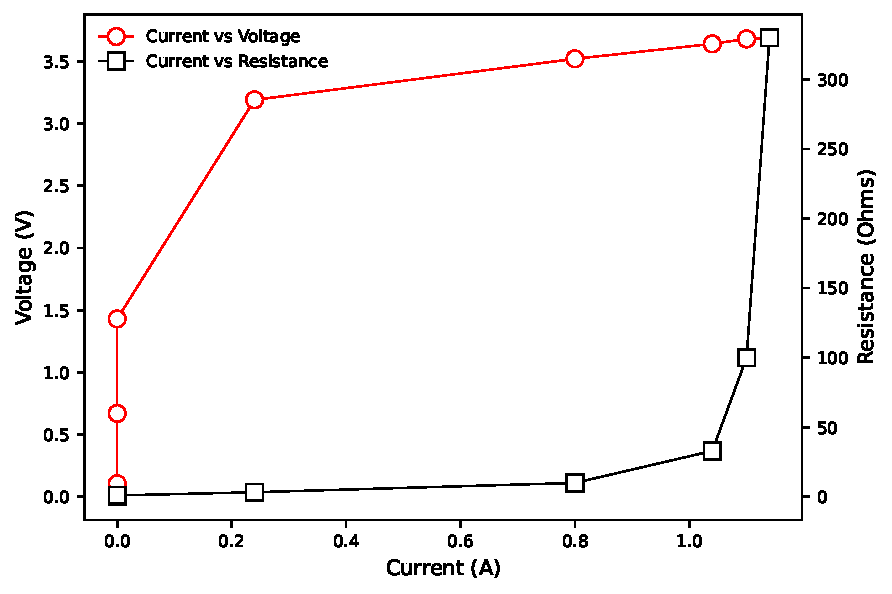
\includegraphics[width=\textwidth]{Output/Exp1.pdf}
        \caption{Voltage vs. Current for Experiment 1.}
        \label{fig:summary_results:exp1}
    \end{subfigure}
    \hfill
    \begin{subfigure}[t]{0.45\textwidth}
        \centering
        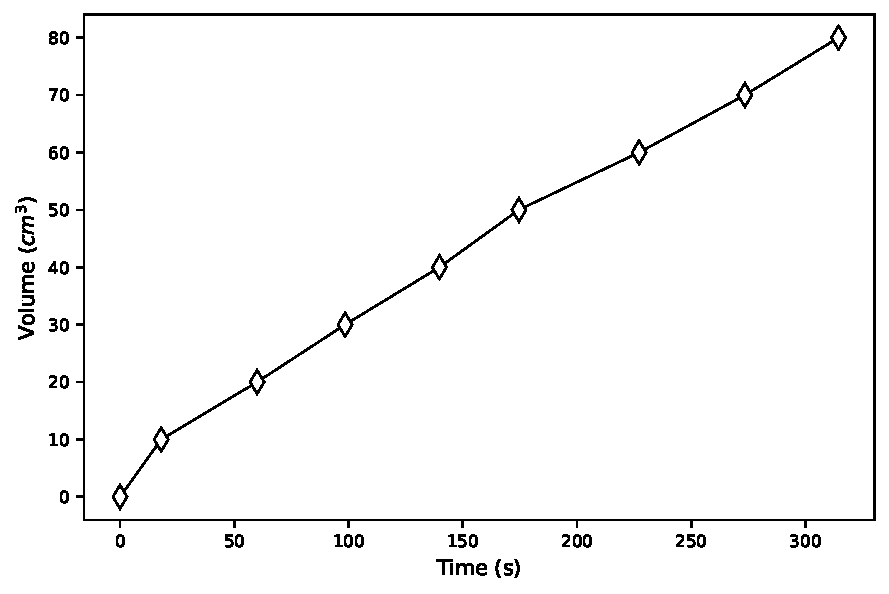
\includegraphics[width=\textwidth]{Output/Exp2.pdf}
        \caption{Time vs. Volume for Experiment 2.}
        \label{fig:summary_results:exp2}
    \end{subfigure}

    \vspace{1cm}  % Optional: Adjust or remove if spacing looks odd

    \begin{subfigure}[t]{0.45\textwidth}
        \centering
        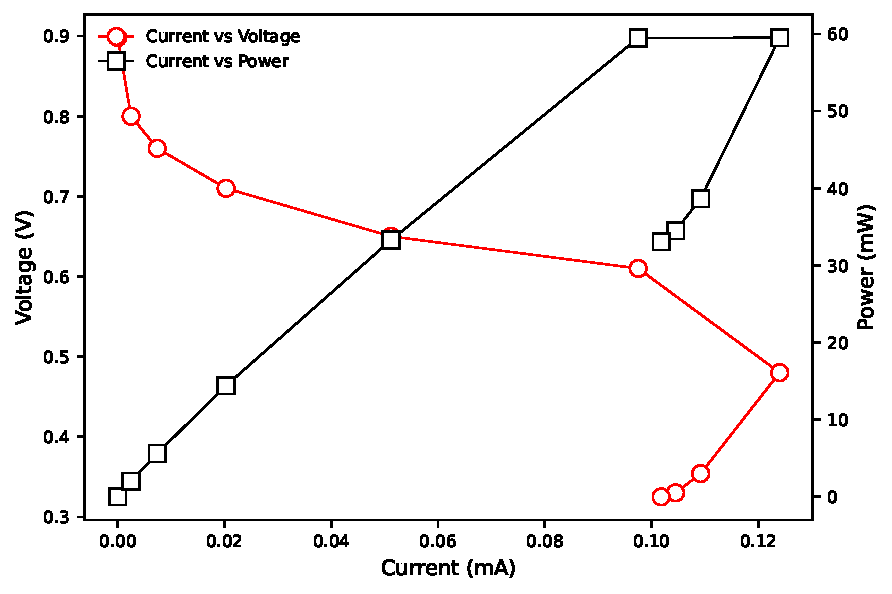
\includegraphics[width=\textwidth]{Output/Exp3_power.pdf}
        \caption{Power vs. Current for Experiment 3.}
        \label{fig:summary_results:exp3}
    \end{subfigure}
    \hfill
    \begin{subfigure}[t]{0.45\textwidth}
        \centering
        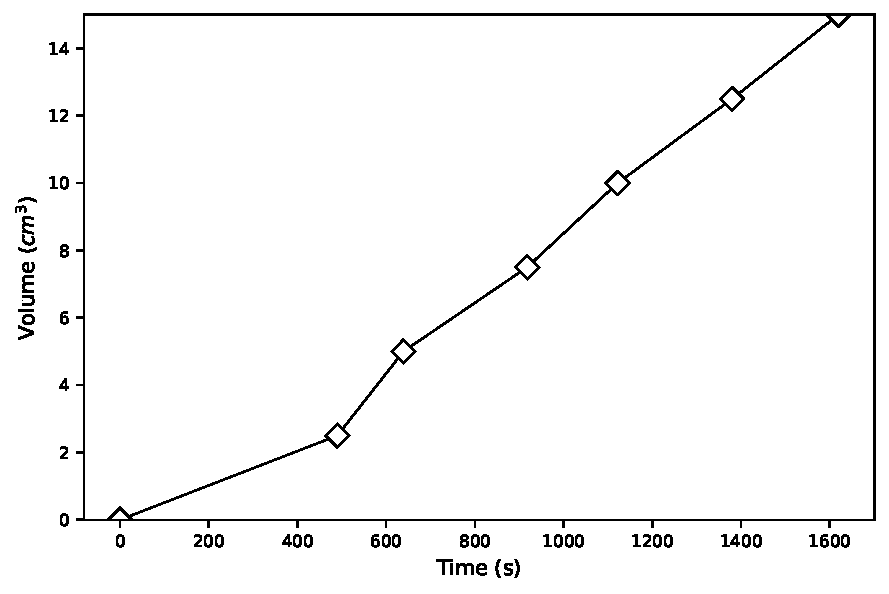
\includegraphics[width=\textwidth]{Output/Exp4.pdf}
        \caption{Time vs. Volume for Experiment 4.}
        \label{fig:summary_results:exp4}
    \end{subfigure}

    \caption{Summary of experimental results for the water electrolyzer and PEM fuel cell.}
    \label{fig:summary_results}
\end{figure}
